\documentclass[11pt]{beamer}
\usetheme{Darmstadt}

% chktex-file 1

\usetheme{Darmstadt}
% More themes at https://www.overleaf.com/learn/latex/Beamer

% --- Packages ---
\usepackage[T1]{fontenc}
\usepackage{lmodern}
\usepackage{amssymb, amsmath}
\usepackage[UKenglish]{datetime}
\usepackage{siunitx} % Writing SI units
\usepackage[most]{tcolorbox}
\usepackage{xcolor}

\newcommand{\mathhighlight}[2]{%
  \tcbhighmath[
    enhanced,
    frame hidden,
    colback=#1,
    boxsep=3pt,
    top=0pt,
    bottom=0pt,
    left=0pt,
    right=0pt,
  ]{#2}
}

\colorlet{highyellow}{yellow!35}
\colorlet{highred}{red!20}
\colorlet{highblue}{cyan!20}
\colorlet{highgreen}{green!20}

\usepackage[
    backend = biber,
    style   = nature,
    isbn    = false
]{biblatex} % BibTeX for bibliography
\usepackage{graphicx, multimedia}

\hypersetup{
    colorlinks=true,
    linkcolor=blue,
    urlcolor=blue,
    citecolor=blue
}

\sisetup{
  per-mode = power
}

% --- Bullet points ---
\setbeamertemplate{itemize item}{\(\bullet\)}
\setbeamertemplate{itemize subitem}{\(\circ\)}
\setbeamercovered{transparent}

% --- Bottom navigation bar ---s
% \setbeamertemplate{navigation symbols}{}
\setbeamertemplate{navigation symbols}{%
    \insertslidenavigationsymbol    % Slide navigation
    \insertframenavigationsymbol    % Frame navigation
    % \insertsubsectionnavigationsymbol    % Subsection navigation
    \insertsectionnavigationsymbol  % Section navigation
    \insertdocnavigationsymbol      % Search / doc navigation
    % \insertbackfindforwardnavigationsymbol % Back/forward arrows

    \usebeamerfont{footline}%
    \usebeamercolor[fg]{footline}%
    \raisebox{1.2pt}[0pt][0pt]{\insertframenumber/\inserttotalframenumber}
}
\setbeamertemplate{sections in toc}[sections numbered]

% --- Custom Commands ---
\newcommand\partialdev[2]{\frac{\partial #1}{\partial #2}}
\newcommand\codev[2]{\frac{D #1}{D #2}}
\renewcommand\d{\mathrm{d}}
\newcommand\dev[2]{\frac{\d #1}{\d #2}}
\newcommand\devsq[2]{\frac{\d^2 {#1}}{\d {#2}^2}}
\addbibresource{bibliography.bib}
\AtBeginBibliography{\scriptsize}

\title{Oceanic Bottom Mixed Layers}
\subtitle{Comparing Ekman and Stokes models for abyssal mixing}
\author{Xing Yu Yi (xyy22), Tian Lang Liu (tll46)}
\institute[Department of Applied Mathematics and Theoretical Physics]{
    Department of Applied Mathematics and Theoretical Physics \\
    University of Cambridge
}
\date{Monday 12th October 2026}
\titlegraphic{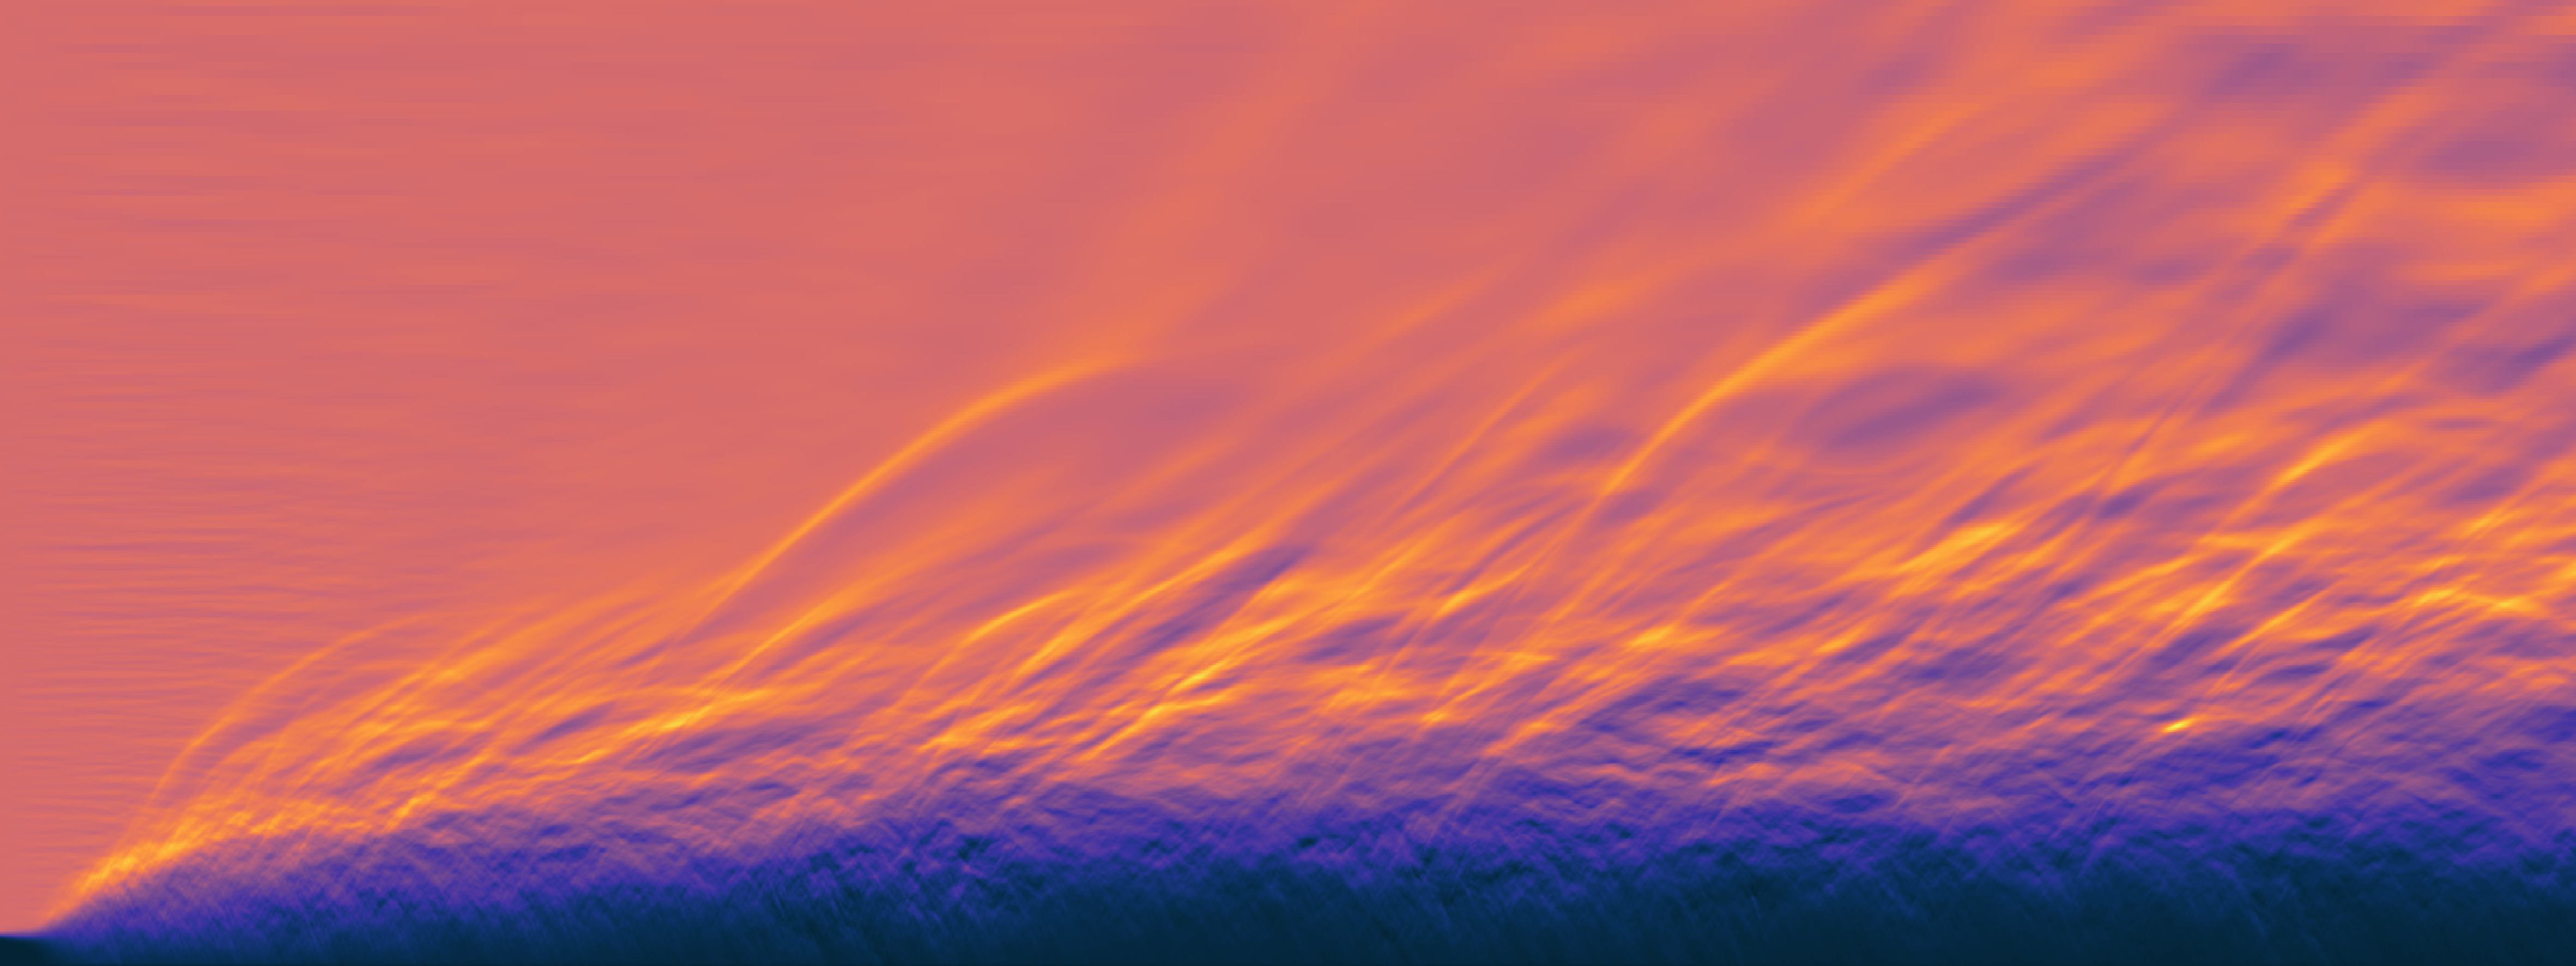
\includegraphics[width=0.42\textwidth]{Figures/Ekman/ekman.png}}

\begin{document}

\maketitle

\begin{frame}{Outline}
    \tableofcontents
\end{frame}

\section{Project aim}

\begin{frame}{What the project actually tested}
    This project was not a single model; it was a comparison of two separate modelling frameworks.

    \begin{itemize}
        \item The Ekman model studies a rotating boundary layer near the bed.
        \item The Stokes model adds wave-induced drift as an extra source of shear and mixing.
        \item Both were analysed with the same diagnostics, so that their turbulent mixing and mixed-layer growth could be compared directly.
    \end{itemize}

    The central question was:
    \[
    \text{Does rotation alone explain the observed abyssal mixed layer, or is wave-induced forcing essential?}
    \]
\end{frame}

\begin{frame}{Observations and motivation}
    Deep-ocean observations show persistent, well-mixed layers just above the seafloor.

    \begin{itemize}
        \item The Hatteras Abyssal Plain provides a classical example \cite{ArmiMillard76}.
        \item Global statistics show especially thick mixed layers in weakly stratified regions \cite{Huang2019}.
        \item The challenge is that the observed layer depth is often much larger than the classical Ekman scale would suggest.
    \end{itemize}

    This is the reason for using two models and then comparing their outcomes.
\end{frame}

\section{Modelling framework}

\begin{frame}{Starting point: rotating Boussinesq flow}
    In a rotating frame, the governing equations are the Boussinesq equations:
    \begin{align}
        \nabla\cdot\mathbf{u} &= 0, \\
        \partial_t\rho + \mathbf{u}\cdot\nabla\rho &= 0, \\
        \partial_t\mathbf{u} + (\mathbf{u}\cdot\nabla)\mathbf{u} + 2\boldsymbol{\Omega}\times\mathbf{u}
        &= -\frac{1}{\rho_0}\nabla p - g\rho'\mathbf{e}_z + \nu\nabla^2\mathbf{u}.
    \end{align}

    The three key ingredients are rotation, viscosity, and buoyancy.
\end{frame}

\begin{frame}{Ekman model}
    Near a rigid boundary, the horizontal momentum balance reduces to
    \[
    -fv = \nu\frac{d^2u}{dz^2}, \qquad fu = \nu\frac{d^2v}{dz^2} + fU_\infty.
    \]

    This is the classical Ekman layer: Coriolis force and viscous stress compete in a thin wall layer.

    The boundary-layer scale is
    \[
    \delta_E = \sqrt{\frac{2\nu}{f}}.
    \]

    In the code, this is the baseline rotating model against which the Stokes model is compared.
\end{frame}

\begin{frame}{Stokes model}
    The Stokes model adds a wave-induced drift $U_s(z)$, which decays with depth like
    \[
    U_s(z) \sim e^{-2kz}.
    \]

    This introduces an additional forcing term in the momentum balance:
    \[
    \partial_t\mathbf{u} + (\mathbf{u}\cdot\nabla)\mathbf{u} + 2\boldsymbol{\Omega}\times\mathbf{u}
    = -\frac{1}{\rho_0}\nabla p + \nu\nabla^2\mathbf{u} + \mathbf{F}_{\mathrm{Stokes}}.
    \]

    The point is that the Stokes forcing can provide additional shear and turbulence near the bed.
\end{frame}

\section{Numerical experiment}

\begin{frame}{What the code does}
    The project uses Oceananigans in Julia and runs the two models separately in a stratified setup.

    \begin{itemize}
        \item the domain is a flat-bottom, geostrophically forced system,
        \item the flow is statistically steady enough to diagnose turbulence,
        \item the mixed layer depth $h(t)$ and turbulence metrics are computed from the output,
        \item the same diagnostic definitions are then used for both models.
    \end{itemize}
\end{frame}

\begin{frame}{The key diagnostic definitions}
    The project uses the same definitions for both datasets, following the code in the repository.

    \begin{itemize}
        \item $\ell = K_T(z=h) / \sqrt{\mathrm{TKE}(z=h)}$
        \item $x = \sqrt{\mathrm{TKE}(z=h)} / N$
        \item $h$ is defined from the pycnocline crossing or peak depending on the chosen configuration
    \end{itemize}

    In the code, this is built carefully because the definition of $h$ matters a lot: different definitions can produce genuinely different values of $K_T$, TKE, and $\ell$.
\end{frame}

\begin{frame}{The important methodological fix}
    A significant part of the project was not just running the models, but making them comparable.

    \begin{itemize}
        \item The original Ekman reduction used resolved buoyancy flux only.
        \item The Stokes model included a subgrid contribution $F_{\mathrm{sgs}}$.
        \item The code also corrected a full-plane versus single-slice averaging issue in the Ekman data.
    \end{itemize}

    In other words, a large part of the project was making sure that the two datasets were actually measuring the same quantity before comparison.
\end{frame}

\section{Results}

\begin{frame}{The comparison result}
    Once both sides were placed on the same footing, the project found that both models are described by a saturating mixing-length law:
    \[
    \ell = L_\infty\left(1-e^{-x/x_0}\right).
    \]

    The important point is that the two flows do not collapse onto the same curve.
\end{frame}

\begin{frame}{The actual fitted values}
    The repository reports the following representative fits for the $T=10\,\mathrm{m}$ case:

    \begin{table}
        \centering
        \begin{tabular}{lccc}
            \hline
            Model & Cases & $L_\infty$ & $x_0$ \\
            \hline
            Stokes & 6 & $0.60\,\mathrm{m}$ & $1.48\,\mathrm{m}$ \\
            Ekman & 7 & $1.79\,\mathrm{m}$ & $5.40\,\mathrm{m}$ \\
            \hline
        \end{tabular}
    \end{table}

    So the Ekman and Stokes models are not equivalent: they produce different asymptotic mixing lengths and different growth rates.
\end{frame}

\begin{frame}{Interpretation}
    This is the main scientific conclusion.

    \begin{itemize}
        \item The Ekman model captures the rotating boundary-layer structure.
        \item It underestimates the strength of the mixing seen in the Stokes-type forcing.
        \item The Stokes model generates stronger turbulent exchange and deeper mixed layers.
        \item The project therefore supports the view that wave-induced forcing matters materially for abyssal mixed-layer growth.
    \end{itemize}
\end{frame}

\begin{frame}{Caveat and uncertainty}
    There is an important caveat in the project logs: several weakly stratified cases were not fully equilibrated.

    \begin{itemize}
        \item in the unconverged cases, $\ell$ was still falling,
        \item so the fitted $L_\infty$ values are partly extrapolations,
        \item the project therefore reports the trend rather than a definitive universal law.
    \end{itemize}

    The key point is not that the two models collapse exactly; it is that they behave differently and the difference is physically meaningful.
\end{frame}

\section{Conclusion}

\begin{frame}{Summary}
    \begin{itemize}
        \item The project compared Ekman and Stokes models separately using the same diagnostics.
        \item The comparison focused on $h$, TKE, $K_T$, and the mixing length $\ell$.
        \item Both models are consistent with a saturating law, but not with the same parameters.
        \item The Stokes model gives stronger mixing and a deeper mixed layer than the Ekman model alone.
        \item The project therefore supports the idea that wave-driven forcing is an important ingredient in abyssal bottom-layer dynamics.
    \end{itemize}
\end{frame}

\begin{frame}{Acknowledgements}
    Many thanks to our supervisors Prof. John Taylor, Dr Bethan Wynne-Cattanach, and Dr Yuchen Ma for their guidance throughout the project.

    \vspace{1em}
    \begin{center}
        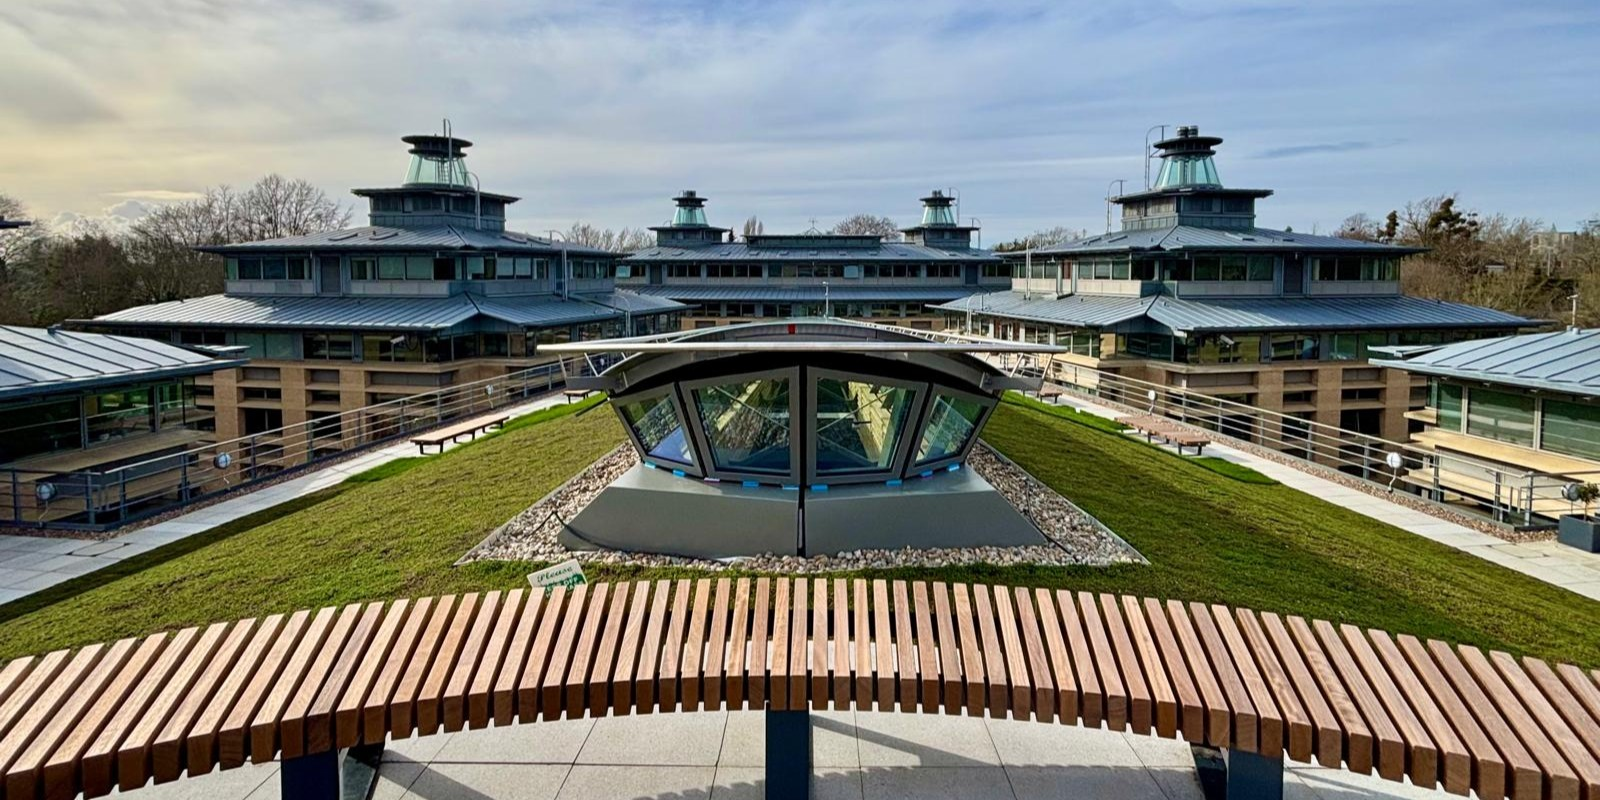
\includegraphics[width=0.55\textwidth]{Figures/cmsrooftop.jpg}
    \end{center}
\end{frame}

\begin{frame}{References}
    \printbibliography[heading=none]
\end{frame}

\end{document}
